\documentclass[11pt,a4paper]{article}
\usepackage{cmap}
\usepackage[utf8]{inputenc}
\usepackage[T1]{fontenc}
\usepackage{lmodern}
\usepackage{microtype}
\usepackage[margin=1.0in]{geometry}
\usepackage{amsmath,amssymb,amsthm,mathtools}
\usepackage{booktabs,array,tabularx}
\usepackage{graphicx}
\usepackage[svgnames]{xcolor}
\usepackage[obeyspaces,spaces,hyphens]{url}
\usepackage[colorlinks=true,linkcolor=DarkBlue,citecolor=DarkBlue,urlcolor=DarkBlue]{hyperref}

\urlstyle{tt}
\def\UrlFont{\ttfamily\upshape\small}
\renewcommand{\arraystretch}{1.25}
\setlength{\tabcolsep}{5pt}

\sloppy
\setlength{\emergencystretch}{4em}

\newtheorem{theorem}{Theorem}[section]
\newtheorem{lemma}[theorem]{Lemma}
\newtheorem{proposition}[theorem]{Proposition}
\theoremstyle{definition}
\newtheorem{definition}[theorem]{Definition}
\newtheorem{remark}{Remark}[section]

\newcommand{\Oz}{\mathcal{O}_0}
\newcommand{\Nrd}{\operatorname{Nrd}}
\newcommand{\lean}[1]{\path{#1}}

\title{\textbf{The Maximal Order of SQIsign's Starting Curve: Machine-Checked Arithmetic in Lean~4, Corrections, and Which Hecke Eigenforms Govern 2-Isogeny Returns to $E_0$}\\[6pt]
\large Edition 2 of ``Post-Quantum Cryptography from the FLT Modular Machinery: Hellegouarch Minimal Weierstrass Semistability, Dual-Isogeny Endomorphism Rings, Half-Integral Deuring Quaternion Orders, and Verified \texttt{SQIsign} in Rust and Lean~4''}
\author{Xavier Callens \\ \small SocrateAI Scientific Research \& Formal Verification Laboratory}
\date{Edition 2, 21 October 2026 (supersedes edition 1, 20 October 2026)}

\begin{document}
\maketitle

\begin{abstract}
Edition~1 of this paper claimed a ``verified SQIsign'' in Rust and Lean~4. An audit on 21 October 2026 found that claim, and two others, to be wrong. The Rust function checks only a reduced norm, and it accepts the scalar $256$, which does not depend on any key or message. The ``non-backtracking response'' $\sigma=128+128j$ lies in $2\Oz$. For the family $(3^p,4^p,3^p+4^p)$, Ribet level lowering does not reach level~$2$: the prime~$7$ always survives. Edition~2 withdraws these claims and labels the remaining Lean results honestly, most of them as constant evaluations or consequences of definitions. It then asks a question about the order $\Oz=\mathbb Z\langle1,i,\tfrac{i+j}2,\tfrac{1+k}2\rangle\subset B_{p,\infty}$ ($p\equiv3\bmod4$), which is $\operatorname{End}(E_0)$ for SQIsign's starting curve $E_0:y^2=x^3+x$. Which weight-2 newforms of level $p$ control $N_e(p)$, the number of primitive elements of reduced norm $2^e$ in $\Oz$, that is, the number of closed non-backtracking $2$-isogeny walks at $E_0$? We measured this in five ways: exact lattice counts; the supersingular 2-isogeny graph over $\mathbb F_{p^2}$; modular-symbol projections of $\theta_{\Oz}$; PARI/GP $L$-values; and Lean~4. The new file \lean{formal/ANSE/PaperC_DeuringSpectrum.lean} passes the axiom gate (20 of 20 theorems clean). It proves the Ihara-circle lemma ($|z|^2=\ell\iff a^2\le4\ell$), the $\Oz$ norm form and its halving lemma, the constant evaluation exhibiting $\sigma$'s coordinates as twice an integral vector, semistability for every inhabited Hellegouarch triple, and $v_7(3^p+4^p)=1+v_7(p)$ with $p\nmid2v_7$ for every prime $p\ge5$. All controls passed. The results:
(i) $N_e(3)=18\cdot2^e$ and $N_e(7)=6\cdot2^e$ hold exactly for $e\le22$.
(ii) For all 13 primes $p\le83$, the minimal recurrence of $N_e$ equals $(x-2)\prod_f x^{d_f}P_f(x+2/x)$ over the orbits that $\theta_{\Oz}$ sees, and every non-trivial root has $|z|^2=2$.
(iii) Over 155 primes $p<2000$ there are 420 cusp orbits. The invisibility of the 211 orbits with root number $-1$ is \emph{not} a test: because $j(E_0)=1728$ is $\mathbb F_p$-rational, Frobenius fixes $e_{E_0}$ and forces the projection to vanish on every $w=-1$ orbit (Section~\ref{sec:w-forced}); it is consistent with Gross's formula but cannot fail. The tested content is the $w=+1$ half: of the 209 orbits with root number $+1$, 21 are invisible, and for every one of these 21, PARI finds $L(f,1)=0$ (9 orbits) or $L(f\otimes\chi_{-4},1)=0$ (12 orbits), as Gross's formula requires. Of the 83 classes examined, 47 have $w=+1$ and carry this content; the other 36 have $w=-1$, where agreement is forced twice over and is not evidence. Edition~3 prices the $w=+1$ agreement and proves the forcing. Visibility agrees with $L$-nonvanishing on all 48 $w=+1$ orbits; under a within-prime permutation null the exact p-value is $1/11520=8.7\times10^{-5}$, and a single discordant orbit would raise it to $1.6\times10^{-3}$, so unlike the permutation control it withdraws, this test can fail. The 21 invisible $w=+1$ orbits are every such orbit in the range, not a sample, and 9 of them have even analytic rank $\ge2$. The forcing of the $w=-1$ half is now a machine-checked theorem rather than a remark (\lean{formal/ANSE/PaperC_ForcedVisibility.lean}, 6 of 6 clean), together with a witness that its hypotheses are non-vacuously satisfiable and a proof that the same hypotheses constrain nothing when $w=+1$.
(iv) The largest eigenvalue seen from $E_0$ is strictly smaller than the global one at 36 of these primes.
No falsification criterion was met. None of this is a new theorem: (i)--(iii) are consequences of Eichler, Deligne and Gross that we test computationally. What is new is the measurement for SQIsign's own maximal order, and the corrections.
\end{abstract}

\tableofcontents

\section*{Correction notice}
\addcontentsline{toc}{section}{Correction notice}
Edition~1 (20 October 2026) made the claims listed below. Edition~2 withdraws or corrects each one, for the reason given. The corrections come from an audit on 21 October 2026. The audit recomputed every constant with PARI/GP~2.17.2~\cite{PARI}, re-ran the Lean gate and \texttt{cargo test}, probed the Rust function with crafted inputs, and checked the cited Lean projects against a fresh clone of \url{https://github.com/ImperialCollegeLondon/FLT}.
\begin{enumerate}
  \item \textbf{Review claims.} The PDF of edition~1 contained no peer-review claim. The pipeline that generated this series of papers, however, also wrote ``multi-round peer review'' files and scores for it. That procedure called no model and involved no reviewer. Its findings were fixed strings, and its scores were pass fractions of local string checks. Any review, score or approval attached to Paper~C is void. This paper has not been peer reviewed.
  \item \textbf{``Verified \texttt{SQIsign} in Rust and Lean~4'', ``zero-gap verification chain'', ``constant-time verifier''.} Withdrawn. \texttt{verify\_sqisign\_response} in \path{sub_projects/socrateai_scientific_quantum_computing/sqisign_flt_verifier/src/lib.rs} takes no public key, message, curve or challenge isogeny, and does no $\mathbb F_{p^2}$ arithmetic. It checks that a quaternion has reduced norm $\ell^e$, together with a few trivial conditions. A probe (Section~\ref{sec:rust}) shows that it accepts the scalar $256$ and edition~1's $\sigma$, both of which are in $2\Oz$. The function contains short-circuit \texttt{\&\&} chains and integer division, so it is not branch-free, and its timing was never measured. None of SQIsign's verification is implemented or verified here.
  \item \textbf{``$\sigma=128+128j$ is a non-backtracking $2^{16}$ response; $\gcd(2^{16},3^8)=1$ prevents backtracking.''} False. In $\Oz$ coordinates $\sigma=(128,-128,256,0)=2\cdot(64,-64,128,0)$, so $\sigma\in2\Oz$ and its walk backtracks. Lean: \lean{paper_sigma_in_two_O0}. Coprimality of $2^{16}$ and $3^8$ says nothing about backtracking within a $2$-power walk. A primitive element of norm $2^{16}$ is given in Theorem~\ref{thm:primitive}.
  \item \textbf{``Ribet level lowering strips all odd prime factors \dots\ obstructing level lowering below $\Gamma_0(2)$'' for $(3^p,4^p,3^p+4^p)$.} False for this family. For every prime $p\ge5$ the prime~$7$ divides $3^p+4^p$ to exponent $1+v_7(p)$, and $p\nmid 2v_7(3^p+4^p)$. So for $p\neq7$, $7$ stays in the Serre level, and for $p=7$ the representation $\bar\rho_7$ is not finite at~$7$. Lean: \lean{seven_survives_serre_level}. PARI gives the Serre levels in Table~\ref{tab:frey}. The canonical witness $(15,16,31)$ even has good reduction at~$2$. The strip-to-level-$2$ argument applies only to genuine Fermat triples, that is, to the empty type \texttt{FreyPackage}.
  \item \textbf{Semistability ``machine-checked for the inhabited package''.} In edition~1 the quantified statement was proved only over \texttt{FreyPackage}, which is empty by Wiles' theorem, so it was vacuous. Edition~2 proves it for every \texttt{InhabitedHellegouarchPackage} (\lean{inhabited_hellegouarch_semistable}).
  \item \textbf{``Strict Pizer Ramanujan spectral gap $4\ell<(\ell+1)^2$''; ``Hecke out-degrees $\{3,3,5,8\}$ at $N=15$''; ``Cerednik--Drinfeld'' theorem name.} Relabelled. $4\ell<(\ell+1)^2$ is $(\ell-1)^2>0$, which holds for every graph. The Ramanujan property is a statement about the non-trivial eigenvalues, proved for these graphs by Pizer~\cite{Pizer1990} from Eichler--Shimura and Deligne, and edition~1 neither formalised nor measured it. Section~\ref{sec:contribution} measures it. The out-degrees follow from the definition \texttt{if l | N then l else l+1}. Level~$15$ plays no role in supersingular isogeny graphs, whose level is $p$. The Lean theorem name has no Cerednik--Drinfeld content.
  \item \textbf{``$98304$ non-backtracking 2-isogeny walks of length 16''.} $3\cdot2^{15}$ counts non-backtracking walks in the 3-regular tree, with any endpoint. The number of closed walks at $E_0$ (cyclic $2^{16}$-endomorphisms, $N_{16}/|\Oz^\times|$) equals $98304$ only for class number one ($p=3,7$). It is $59136$ at $p=11$, $13824$ at $p=43$ and $7052$ at $p=83$ (Section~\ref{sec:contribution}).
  \item \textbf{$\Nrd_{313,1}(3,2,1,1)=639$ presented as $B_{313,\infty}$ data.} $313\equiv1\bmod4$, and PARI finds $(-1,-313)_\mathbb Q$ ramified at $\{2,\infty\}$ (Hilbert symbols $-1$ at $2$, $+1$ at $313$). This is a Hamilton-type algebra, not $B_{313,\infty}$. The value $639$ is correct, but the example is outside the theorem's scope, and it is used below as a negative control.
  \item \textbf{Non-coprime triple $(3,6,9)$: ``$c_4=63$''.} The $u=2$ model is not integral here. PARI gives the minimal model $[0,0,0,-21,20]$ with $c_{4,\min}=1008$, $\Delta_{\min}=419904$ and conductor $288=2^5\cdot3^2$. The reduction is additive at both $2$ and $3$. The conclusion ``additive at~$3$'' stands.
  \item \textbf{``Lipschitz suborder of index 2 or 4''; ``maximal Hurwitz/Deuring order''.} The index is exactly $4$: the Gram determinants are $16p^2$ and $p^2$, verified by PARI for $p=3,7,11,311,331$. ``Hurwitz order'' refers to $B_{2,\infty}$. We call $\Oz$ the standard maximal order containing $\mathbb Z[i]$.
  \item \textbf{\texttt{DualIsogenyAPI}, \texttt{DualEndData}, \texttt{IsDualPair} attributed to the Imperial College FLT project.} They are not in \url{https://github.com/ImperialCollegeLondon/FLT}: a grep of a fresh clone finds none of them. They are local to this repository. \texttt{FreyPackage} does exist there, in \path{FLT/FreyCurve/FreyPackage.lean}. The blueprint is titled ``Towards a Lean proof of Fermat's Last Theorem''~\cite{BuzzardTaylor}. The local file \path{sub_projects/socrateai_scientific_quantum_computing/formal/FLT_Def_DualIsogenyAPI.lean} uses the banned \texttt{import Mathlib} and has no \texttt{\#print axioms} lines, so the gate leaves all 40 of its declarations unchecked. \path{formal/ANSE/MensuraElenchusThreeMissions.lean} is unchecked for the same reason (18 declarations), and the composition-degree theorem it holds is proved by \texttt{rfl}. Edition~2 cites neither file as verified.
  \item \textbf{Table~1 ``verification layer'' and edition~1's Figures~1--2.} The table now states what kind of fact each theorem is (Table~\ref{tab:kinds}). Edition~1's figures plotted definitional formulas. Its Fig.~2(a) also illustrated the wrong Ribet claim. Both figures are removed.
\end{enumerate}

\section{Introduction}
Isogeny-based signatures such as SQIsign~\cite{DeFeo2020,SQIsignSpec} translate walks in the supersingular $\ell$-isogeny graph over $\mathbb F_{p^2}$ into ideals and elements of a maximal order of the definite quaternion algebra $B_{p,\infty}$. This translation is Deuring's correspondence~\cite{Deuring1941,Kohel1996,Voight}. SQIsign starts from $E_0:y^2=x^3+x$ with $p\equiv3\bmod4$, whose endomorphism ring is
\[
\Oz=\mathbb Z+\mathbb Zi+\mathbb Z\tfrac{i+j}{2}+\mathbb Z\tfrac{1+k}{2}\subset B_{p,\infty}=\Big(\tfrac{-1,-p}{\mathbb Q}\Big).
\]
Edition~1 formalised arithmetic of $\Oz$ and of Frey--Hellegouarch curves in Lean~4 and paired it with a Rust crate. Edition~2 keeps the correct part of that work (Section~\ref{sec:formal}), states plainly what the Rust crate does (Section~\ref{sec:rust}), and adds a measurement (Section~\ref{sec:contribution}). The measurement asks which Hecke eigenforms of level~$p$ actually govern the closed non-backtracking 2-isogeny walks at $E_0$. Section~\ref{sec:frey} corrects the level-lowering statement for the Frey family. Sections~\ref{sec:scope}--\ref{sec:directions} give the scope, the limitations and open directions.

\paragraph{Gate.} The only accepted Lean check is \texttt{.venv/bin/python -m anse.formal.lean\_runner <file>}. It compiles the file, requires a \texttt{\#print axioms} line for every theorem, and rejects \texttt{sorryAx} and any axiom outside $\{$\texttt{propext}, \texttt{Classical.choice}, \texttt{Quot.sound}$\}$. The toolchain is \path{leanprover/lean4:v4.34.0-rc2} with Mathlib~\cite{Mathlib}, imported module by module, never through \texttt{import Mathlib}.

\section{Edition-1 results that stand, and what kind of fact each is}
\label{sec:formal}
The five edition-1 theorems in \path{formal/ANSE/Breakthroughs3Domains.lean} pass the gate: that file has 26 declarations, all 26 clean, re-run on 21 October 2026 and recorded in \path{paper_c_v2_lean_gate.json}. The file is shared with other papers and was not edited. Table~\ref{tab:kinds} states what each theorem actually proves.

\begin{table}[htbp]
\centering
\caption{Edition-1 Lean theorems (all gate-clean) and the kind of fact each one is.}
\label{tab:kinds}
\footnotesize
\begin{tabularx}{\textwidth}{@{}l X l@{}}
\toprule
\textbf{Lean declaration} & \textbf{Content actually proved} & \textbf{Kind} \\
\midrule
\texttt{P1\_T1\_inhabited\_hellegouarch\_\dots} & $c_4,\Delta$ values at $(15,16,31)$; $(4p-8)\bmod p$ arithmetic; semistability and Ribet parts quantified over the empty \texttt{FreyPackage} & constant evaluation; vacuous parts \\
\texttt{P1\_T2\_flt\_dual\_isogeny\_api\_\dots} & $\operatorname{Tr}(a+b\phi)^2-4\operatorname N(a+b\phi)=b^2(t^2-4n)$; values at $(128,128,0,3)$ & polynomial identity; constant evaluation \\
\texttt{P1\_T3\_deuring\_quaternion\_\dots} & $\Nrd_{p,q}$ multiplicative; $\Oz$ norm integral for $p=4m+3$ & substantive (elementary) identities \\
\texttt{P1\_T4\_cerednik\_drinfeld\_\dots} & $4\ell<(\ell+1)^2$; \texttt{decide} on the out-degree definition at $N=15$; $3\cdot2^{15}=98304$ & trivial inequality; definition consequence \\
\texttt{P1\_T5\_sqisign\_challenge\_\dots} & associativity of integer products; $65536\cdot6561=429981696$; two B\'ezout identities & ring identity; constant evaluation \\
\bottomrule
\end{tabularx}
\end{table}

\begin{theorem}[Frey--Hellegouarch witness $(15,16,31)$; edition~1 Thm.~2.1, corrected]
\label{thm:frey}
For $A+B=C$, $\gcd(A,B)=1$, $A\equiv3\bmod4$ and $16\mid B$, the curve $Y^2=X(X-A)(X+B)$ has, after $X=4x$, $Y=8y+4x$, the integral model $y^2+xy=x^3+\frac{B-1-A}4x^2-\frac{AB}{16}x$, with $c_{4}=C^2-AB$ and $2^8\Delta=(ABC)^2$. At $(15,16,31)$ this is $y^2+xy=x^3-15x$, with $c_4=721$ and $\Delta=216225=3^2\cdot5^2\cdot31^2$. The B\'ezout identities $694\cdot55353600-53280719\cdot721=1$ and $298\cdot216225-89369\cdot721=1$ hold. PARI confirms that this model is minimal, has conductor $465=3\cdot5\cdot31$ with multiplicative (Kodaira $I_n$) reduction at $3,5,31$, and has good reduction at~$2$. For every inhabited triple and every prime $q$, $q\mid ABC\Rightarrow q\nmid C^2-AB$. Lean: \lean{inhabited_hellegouarch_semistable} in \lean{formal/ANSE/PaperC_DeuringSpectrum.lean}, with the positive control \lean{witness_semistable_at_31} and the negative control \lean{noncoprime_triple_not_semistable} for $(3,6,9)$.
\end{theorem}
\noindent Minimality and multiplicative reduction are the classical computation, confirmed by PARI for $(15,16,31)$. They are not formalised.

\begin{theorem}[Norms on $\Oz$; edition~1 Thm.~2.3]
\label{thm:o0}
Let $p=4m+3$. In the basis $(1,i,\frac{i+j}2,\frac{1+k}2)$ the reduced norm is $Q_m(x)=x_0^2+x_1^2+(m+1)(x_2^2+x_3^2)+x_0x_3+x_1x_2$. It satisfies $4Q_m(x)=(2x_0+x_3)^2+(2x_1+x_2)^2+p(x_2^2+x_3^2)$ (\lean{o0Norm_four_mul}), which is edition~1's half-integral formula with $a=2x_0+x_3$, $b=2x_1+x_2$, $c=x_2$, $d=x_3$. It is positive definite (\lean{o0Norm_pos}) and $Q_m(2x)=4Q_m(x)$ (\lean{o0Norm_two_smul}). Hence $Q_m(2y)=4n\iff Q_m(y)=n$ (\lean{o0Norm_half}), and the number of primitive elements ($x\notin2\Oz$) of norm $4n$ is $r(4n)-r(n)$. The norm is multiplicative on $B_{p,\infty}$ (edition~1, \lean{P1_T3_deuring_quaternion_order_norm_multiplicativity}).
\end{theorem}

\begin{theorem}[Edition~1's $\sigma$ is not primitive; a primitive replacement]
\label{thm:primitive}
In $\Oz\subset B_{3,\infty}$, edition~1's $\sigma=128+128j$ has coordinates $(128,-128,256,0)=2\cdot(64,-64,128,0)$ and norm $65536=4\cdot16384$ (\lean{paper_sigma_in_two_O0}). The scalar $256$ has coordinates $(256,0,0,0)\in2\Oz$ (\lean{scalar_256_in_two_O0}). Both Lean declarations are \emph{constant evaluations} in this paper's vocabulary: they state norm equalities on literal coordinate vectors whose entries are visibly even, not a membership statement of the form $\exists y,\ x=2\cdot y$. The membership is immediate from the displayed coordinates, but it is the reader, not the kernel, who takes that step. The element $247+5i+2\cdot\frac{i+j}2+17\cdot\frac{1+k}2=\frac{511}2+6i+j+\frac{17}2k$ has norm $2^{16}$ and is primitive (\lean{primitive_sigma_witness}). It is the primitive element with the smallest coordinate sum among those with non-negative coordinates (enumeration in the experiment script). There are $1179648=18\cdot2^{16}$ primitive elements of norm $2^{16}$ in all (lattice count, Section~\ref{sec:contribution}).
\end{theorem}

\noindent The identities of edition~1's Theorem~2.2 for $\mathbb Z[\phi]$ ($\operatorname{Tr}(a+b\phi)=2a+tb$, $\operatorname N(a+b\phi)=a^2+tab+nb^2$, discriminant $b^2(t^2-4n)$) are correct polynomial identities and are kept as such. Degree multiplicativity of composed dual pairs is definitional (\texttt{rfl}) in an ungated local file, and it is not claimed as verified.

\section{The Rust crate: what it checks, and a negative control}
\label{sec:rust}
\texttt{cargo test --release} on \path{sqisign_flt_verifier} passes 6 of 6 tests. Those tests compare constants. To find out what \texttt{verify\_sqisign\_response(q, 2, 16, 6561)} accepts, we call it from a probe crate, \path{scripts/three_breakthroughs/paper_c_v2_rust_probe}. Table~\ref{tab:probe} shows the results. Every input with norm $2^{16}$ is accepted, whether it is primitive or lies in $2\Oz$. Only the wrong-norm input is rejected. The function is therefore a norm check, and we recommend renaming it (e.g.\ \texttt{norm\_degree\_check}). It is not a signature verifier.

\begin{table}[htbp]
\centering
\caption{\texttt{verify\_sqisign\_response(q, 2, 16, 6561)} on elements $a+bi+cj+dk$ of $B_{3,\infty}$ (real output of the probe crate, recorded in \texttt{paper\_c\_v2\_results.json}).}
\label{tab:probe}
\footnotesize
\begin{tabular}{@{}l c c c c@{}}
\toprule
\textbf{input} & $(a,b,c,d)$ & $\Nrd$ & \textbf{in $2\Oz$?} & \textbf{accepted} \\
\midrule
edition~1's $\sigma=128+128j$ & $(128,0,128,0)$ & $65536$ & yes & true \\
scalar $256=[2]^8$ & $(256,0,0,0)$ & $65536$ & yes & true \\
$128+128k$ & $(128,0,0,128)$ & $65536$ & yes & true \\
primitive $1+23j+146k$ & $(1,0,23,146)$ & $65536$ & no & true \\
wrong norm & $(255,1,1,0)$ & $65029$ & -- & false \\
\bottomrule
\end{tabular}
\end{table}

\section{Contribution: which Hecke eigenforms govern 2-isogeny returns to $E_0$}
\label{sec:contribution}

\subsection{Question and predictions}
By Deuring's correspondence, a cyclic $2^e$-isogeny $E_0\to E_0$ is the same thing as a primitive $\alpha\in\Oz$ with $\Nrd(\alpha)=2^e$, up to the unit group $\Oz^\times=\operatorname{Aut}(E_0)$. Here primitive means $\alpha\notin2\Oz$, which is the same as saying the walk does not backtrack. We study
\begin{align*}
N_e(p)&=\#\{\alpha\in\Oz\setminus2\Oz:\Nrd(\alpha)=2^e\}=r(2^e)-r(2^{e-2})\quad(e\ge2),\\
r(n)&=\#\{\alpha\in\Oz:\Nrd\alpha=n\},
\end{align*}
where the second equality is Theorem~\ref{thm:o0}. The theta series $\theta_{\Oz}=\sum_n r(n)q^n$ is a weight-2 form on $\Gamma_0(p)$. It splits into an Eisenstein part, fixed by the Eichler mass formula, and a cusp part supported on some of the newform Galois orbits $f$ of level $p$. We call those orbits \emph{visible}. The question is: \textbf{which orbits are visible from $E_0$, and what do they do to the return counts?} We fixed the following predictions before the full run.
\begin{itemize}
  \item[\textbf{P1}] $N_e(p)=36\cdot2^e/(p-1)+O_p(2^{e/2})$, exactly for class number one ($p=3$: $18\cdot2^e$; $p=7$: $6\cdot2^e$).
  \item[\textbf{P2}] The minimal linear recurrence of $(N_e)_{e\ge2}$ has characteristic polynomial $(x-2)\prod_{f\text{ visible}}x^{d_f}P_f(x+2/x)$, where $P_f$ is the characteristic polynomial of $a_2$ on the orbit. Every non-trivial root then satisfies $|z|^2=2$ exactly when $a_f(2)^2\le8$, by the Ihara-circle lemma (Theorem~\ref{thm:ihara}).
  \item[\textbf{P3}] (Gross~\cite{Gross1987}.) $f$ is visible iff $L(f,1)L(f\otimes\chi_{-4},1)\ne0$. In particular no orbit with root number $w=-1$ is visible, and an orbit with $w=+1$ is invisible only when one of the two central values vanishes.
\end{itemize}
P1--P3 are consequences of known theorems (Eichler--Shimura and Deligne for the error term, Gross for P3). We do not claim to prove anything new. We claim to test them, in data and from five independent directions, for the maximal order that SQIsign uses. P1, P2 and the $w=+1$ half of P3 could each have failed in our data through a pipeline error or a wrong dictionary. The $w=-1$ half could not, for the reason we now give.

\paragraph{The $w=-1$ half of P3 is forced, not tested.}\label{sec:w-forced}
Our base point is $E_0$ with $j=1728$. That value lies in $\mathbb F_p$, so the Frobenius permutation $F:j\mapsto j^p$ of the supersingular set fixes the corresponding basis vector: $Fe_{E_0}=e_{E_0}$. $F$ commutes with every Brandt matrix --- our pipeline verifies this numerically for $B(2)$ at every prime, and it holds for the higher $B(\ell)$ used at the 15 primes where $B(2)$ alone does not separate the orbits --- and on the $f$-component it acts by the scalar $a_f(p)=-\varepsilon_p=w$. Writing $\pi_f$ for the projection onto that component,
\[
  \pi_f e_{E_0}=\pi_f F e_{E_0}=F\pi_f e_{E_0}=w\,\pi_f e_{E_0},
\]
so $w=-1$ gives $\pi_f e_{E_0}=0$: every root-number-$-1$ orbit is invisible from \emph{this} base point by a one-line argument, for every $p$, whatever the central values do. The same holds for the M4 cross-check, since $\theta_{\Oz}$ is a $W_p$-eigenform for the same reason. In our implementation the conclusion is literal rather than measured: in \texttt{brandtvis}, a visible orbit's witness is $u=\pi_f e_{E_0}$ with $Fe_{E_0}=e_{E_0}$, hence $Fu=u$ and the recorded sign is $+1$ by construction. The count ``0 of 211 visible'' is therefore an identity of the pipeline, and we report it as a consistency check on the pipeline, not as evidence for Gross's formula. The root numbers of the invisible orbits are recovered from a different basis vector and are genuine; what is not a measurement is the implication $w=-1\Rightarrow$ invisible.

There is a second, independent reason the same implication cannot fail, and it does not involve the base point at all: when $w=-1$ the functional equation is odd, so $L(f,1)=0$ automatically, and Gross's criterion therefore predicts invisibility of every $w=-1$ orbit from \emph{any} base point. The two forcings compound. A base point outside $\mathbb F_p$ removes the Frobenius one and makes the observation a genuine, if weak, test of the Deuring--Gross dictionary --- a visible $w=-1$ orbit would refute it --- but the prediction being tested is still vanishing, not non-vanishing. By the same token, the symmetry between the two root-number classes in our results table is apparent only: the $w=+1$ row records a measurement and the $w=-1$ row records two theorems.

\subsection{Lean~4 theorems (file \texttt{formal/ANSE/PaperC\_DeuringSpectrum.lean})}
\begin{theorem}[Ihara circle; \lean{ihara_circle}, \lean{ihara_circle_coords}]
\label{thm:ihara}
Let $\ell>0$ and $a$ be real, and let $z\in\mathbb C$ satisfy $z^2-az+\ell=0$. Then $|z|^2=\ell\iff a^2\le4\ell$.
Controls: \lean{ihara_positive_control_11a} ($a=-2$, the eigenvalue $a_2$ of $11a$: every root of $z^2+2z+2$ has $|z|^2=2$) and \lean{ihara_negative_control} ($a=3$: the root $z=1$ of $z^2-3z+2$ is off the circle).
\end{theorem}
\noindent This lemma turns ``all recovered roots have modulus $\sqrt2$'' into ``all visible $a_f(2)$ satisfy the Ramanujan bound $|a|\le2\sqrt2$''. It does not prove the bound, which is Deligne's theorem and is not formalised.

\begin{theorem}[Serre level of the Frey family; \lean{seven_survives_serre_level}]
\label{thm:seven}
For every prime $p\ge5$, $v_7(3^p+4^p)=1+v_7(p)$ and $p\nmid2\,v_7(3^p+4^p)$. (Lifting the exponent via Mathlib's \texttt{padicValNat.pow\_add\_pow}; also \lean{seven_dvd_three_pow_add_four_pow}: $7\mid3^n+4^n$ for odd $n$.)
\end{theorem}

\noindent The file also holds Theorems~\ref{thm:frey}--\ref{thm:primitive} above, and decide-checked class-number-one counts at $p=3$. These say that the box $[-3,3]^4$ contains every element of norm $\le4$ (\lean{norm_box_p3}), that $|\Oz^\times|=12$ (\lean{unit_count_p3}), $N_1=36$ (\lean{primitive_count_p3_e1}) and $N_2=84-12=72$ (\lean{primitive_count_p3_e2}). This verifies $N_e(3)=18\cdot2^e$ in the kernel for $e=1,2$ only, not for all~$e$. One step in that chain is informal: no theorem links the enumerator \lean{count3} to the cardinality of $\{x:Q_0(x)=n\}$. \lean{norm_box_p3} bounds where the solutions can lie, and \lean{count3} enumerates that box, but the identification of the enumeration with the count is read off the definition rather than proved, exactly as with the \texttt{Finset} bijection below.

\paragraph{Gate result (real output).} \texttt{.venv/bin/python -m anse.formal.lean\_runner formal/ANSE/PaperC\_DeuringSpectrum.lean} exits~0: 20 theorems declared, 20 clean, no \texttt{sorryAx}, and only the axioms \texttt{propext}, \texttt{Classical.choice} and \texttt{Quot.sound}. The file has 24 \texttt{\#print axioms} lines, one for every declaration including its 4 definitions. The imports are \texttt{Mathlib.Tactic}, \texttt{Mathlib.Analysis.InnerProductSpace.Basic}, \texttt{Mathlib.NumberTheory.Multiplicity} and \texttt{ANSE.ElenchusTrilogySpec}. The planned general bijection statement $N_e=r(2^e)-r(2^{e-2})$ as a \texttt{Finset} equality was not proved. The halving lemma \lean{o0Norm_half} is the weaker statement we did prove, and the count identity above uses it together with the map $x\mapsto2x$ outside Lean.

\subsection{Lean~4: the forcing argument itself (file \texttt{formal/ANSE/PaperC\_ForcedVisibility.lean})}\label{sec:lean-forced}
Edition~2 withdrew the $w=-1$ half of P3 on the strength of the prose argument in Section~\ref{sec:w-forced}. A withdrawal that rests on a remark is weaker than the claim it retracts, so this edition proves the argument instead. The new file passes the same gate (6 declarations, 6 clean, no \texttt{sorryAx}, axioms $\{$\texttt{propext}, \texttt{Classical.choice}, \texttt{Quot.sound}$\}$; imports \texttt{Mathlib.Tactic}, \texttt{Mathlib.Algebra.Module.LinearMap.Basic}, \texttt{Mathlib.Data.Real.Basic}).

\begin{itemize}
  \item \lean{frobenius_forces_vanishing}: for linear $F,\pi$ on a module over a field in which $2\ne0$, if $Fe_0=e_0$, $\pi F=F\pi$ and $F\pi=w\pi$ with $w=-1$, then $\pi e_0=0$. This is the one-line argument of Section~\ref{sec:w-forced}, stated so that nothing arithmetic can enter: the conclusion follows from the three hypotheses and $2\ne0$ alone. Our ``0 of 211'' is this theorem instantiated 211 times, not 211 opportunities to fail.
  \item \lean{frobenius_forcing_hypotheses_are_satisfiable_nontrivially}: a witness over $\mathbb Q^2$ with $e_0\ne0$ and $\pi\ne0$ satisfying all three hypotheses. Without it the previous theorem could hold vacuously, and a vacuous forcing theorem would not justify withdrawing anything.
  \item \lean{frobenius_forces_nothing_at_w_one}: with $w=+1$ the same hypotheses are met both by a configuration with $\pi e_0\ne0$ and by one with $\pi e_0=0$. So the $w=+1$ stratum is not constrained by the forcing, which is the formal content of the claim that the measurement lives there.
  \item \lean{odd_functional_equation_forces_central_zero}: if $L(s)=w\,L(2-s)$ for all $s$ and $w=-1$ then $L(1)=0$; with \lean{even_functional_equation_permits_nonzero} as its control. This is the second, base-point-independent forcing: it shows that moving the base point off $\mathbb F_p$ would not by itself restore content to the $w=-1$ half, because Gross's criterion would still predict invisibility through $L(f,1)=0$.
\end{itemize}

What is \emph{not} formalised here is that the Brandt operators and Frobenius satisfy these hypotheses on the supersingular basis; that is Deuring--Eichler theory together with the numerical commutation check the pipeline performs at each prime. The theorems are conditional on it, and the file says so. Their role is narrow and worth stating precisely: they establish that \emph{if} the standard dictionary holds, then the $w=-1$ observation could not have come out otherwise --- which is exactly what a reader needs in order to discount it.

\subsection{Computation}
The script is \path{scripts/three_breakthroughs/paper_c_v2_experiment.py}. All number-theoretic ground truth comes from PARI/GP~2.17.2 through \path{paper_c_v2_pari_worker.py}. One run took $633$\,s on 8 cores and wrote \path{paper_c_v2_results.json}.
\begin{description}
  \item[M1] Exact lattice counts $r(2^e)$ for $\Oz$ (numpy integer arithmetic over two-square tables), for the 13 primes $p\equiv3\bmod4$, $p\le83$, and $e\le22$.
  \item[M2] The supersingular 2-isogeny graph over $\mathbb F_{p^2}$, found by breadth-first search from $j=1728$ with \texttt{polmodular(2)} and factoring over $\mathbb F_{p^2}$. Its adjacency matrix is the Brandt matrix $B(2)$. Then $r(2^e)=|\Oz^\times|\,(B(2^e))_{E_0E_0}$ with $B(2^{k+1})=B(2)B(2^k)-2B(2^{k-1})$, extended to $e\le48$.
  \item[M3] Visibility on the graph. The Hecke orbits are the irreducible factors of the characteristic polynomial of $B(2)$; where $B(2)$ alone does not separate them we add $B(3),B(5),\dots$. An orbit is visible iff its projection of $e_{E_0}$ is non-zero. Frobenius $j\mapsto j^p$ acts as $T_p$, so its eigenvalue is $a_p=-\varepsilon_p=w$. Run for all 155 primes $p\equiv3\bmod4$ below $2000$.
  \item[M4] Independent visibility for $p<700$ (65 primes): $\theta_{\Oz}$ from \texttt{qfrep}, minus $\frac{24}{p-1}E_2^{(p)}$, expressed in the $q$-expansions of the newform orbits from modular symbols (\texttt{msinit}, \texttt{mssplit}, \texttt{msqexpansion}, \texttt{msatkinlehner}) up to the Sturm bound.
  \item[M5] $L(f,1)$ and $L(f\otimes\chi_{-4},1)$ for every embedding of every orbit of dimension $\le3$ (PARI \texttt{mfsplit}, \texttt{mfcoefs}, \texttt{lfun}), at 38 digits, with every functional-equation check below $-30$ bits. This was done for all $p<400$ and for every prime with an invisible $w=+1$ orbit (53 primes).
\end{description}
For P2 we ran Berlekamp--Massey over $\mathbb Q$ on $(N_e)_{e\ge2}$ and compared the result with the prediction built from M4's visible orbits. Literature anchors: $a_2(11a)=-2$ and $L(11a,1)=0.2538\ldots$ (LMFDB 11.2.a.a~\cite{LMFDB}); the mass formula and Deuring dictionary~\cite{Voight}; the choice of $E_0$ in SQIsign~\cite{SQIsignSpec}.

\subsection{Controls}
All controls were evaluated before any result was reported, and all passed. Edition~2 carried a caveat here: its \texttt{controls\_ok} gate, and hence the verdict string, still contained the permutation test that edition~2 withdrew in its own text, so the quoted verdict was conditioned on a control the paper disowned. This edition removes it. The gate now rests on the $w=+1$ stratum test of Section~\ref{sec:wplus}, which is falsifiable, and the experiment was rerun from scratch (633\,s, 8 cores) with that gate in place. The withdrawn permutation statistic survives in the results JSON marked \texttt{"informative": false} with the reason attached, as a descriptive record only.

One caveat remains, as in the companion papers: the criteria were fixed in the script's docstring before the runs but the script was untracked in git at the time, so their precedence rests on that docstring and on file timestamps rather than on a commit. The edition-3 amendments to that docstring --- the withdrawal of criterion~(c), the addition of (c$'$) and of positive control~(vii) --- are dated and labelled in place, so the record shows what changed rather than reading as though it had always said so.

\begin{table}[htbp]
\centering
\caption{Positive and negative controls (real output).}
\label{tab:controls}
\footnotesize
\begin{tabularx}{\textwidth}{@{}l X X@{}}
\toprule
\textbf{Control} & \textbf{Requirement} & \textbf{Outcome} \\
\midrule
P(i) class number one & $N_e(3)=18\cdot2^e$, $N_e(7)=6\cdot2^e$, $1\le e\le22$; $|\Oz^\times|=12$ at $p=3$, else 4 & exact for all $e$; units as required \\
P(ii) independent counts & PARI \texttt{qfrep} $=$ numpy ($e\le11$); graph $=$ lattice ($e\le22$); $\#$vertices $=\dim S_2+1$ & equal at all 13 primes \\
P(ii') two visibility methods & M3 $=$ M4 orbit by orbit (charpoly, sign, visibility) & equal at all 65 primes $p<700$ \\
P(iii) known eigenvalue & $p=11$: factor $x^2+2x+2$ ($a_2=-2$); $L(11a,1)=0.25384\ldots$ & recovered; $0.2538418608559107$ \\
P(iv) Gross at $p=139$ & invisible $a_2=1$ orbit has a vanishing central value & $L(f,1)=1.73969$, $L(f\otimes\chi_{-4},1)=-6.7\times10^{-42}$ \\
P(v) Frey $(15,16,31)$ & conductor $465$, $\Delta_{\min}=216225$ & $465$, $216225$ \\
P(vi) visible $w=+1$ orbits & $L(f,1)L(f\otimes\chi,1)\ne0$ & 26 classes, all non-vanishing \\
P(vii) $w=+1$ stratum & \emph{replaces N(iv) in the gate}: visibility must agree with $L$-nonvanishing where nothing forces it, at exact $p<10^{-3}$ & 48 of 48 orbits concordant; $p=1/11520=8.7\times10^{-5}$ within primes; one discordant orbit would give $1.6\times10^{-3}$ and fail (Section~\ref{sec:wplus}) \\
\midrule
N(i) Lipschitz order, $p=3$ & must fail the exact law & $N_{1..6}=4,16,48,96,192,384$ vs.\ $36,72,\dots,1152$: fails \\
N(ii) $(-1,-313)$ & \emph{sanity check, not a control}: $N_e=0$ is forced by a parity argument mod $8$, so it cannot fail & ramified at $\{2,\infty\}$; $N_e=0$ for $2\le e\le22$, as forced \\
N(iii) $\sigma$, scalar 256 & non-primitive; an honest check must reject them & both in $2\Oz$; the Rust function accepts both (Table~\ref{tab:probe}) \\
N(iv) permutation test & \emph{withdrawn}: the shuffle statistic tests an identity of the pipeline, not the data (Section~\ref{sec:w-forced}) & no inferential content; removed from the \texttt{controls\_ok} gate in this edition, kept in the JSON as \texttt{"informative": false}, and replaced there by P(vii) \\
N(v) $(3,6,9)$ & not semistable & conductor $288=2^5 3^2$, additive at 2 and 3 \\
\bottomrule
\end{tabularx}
\end{table}

\subsection{Results}
\paragraph{P1.} The class-number-one laws hold exactly. For the other 11 primes, the normalised deviation $D_e(p)=(N_e-36\cdot2^e/(p-1))/2^{e/2}$ stays bounded: $\max|D_e|\le5.143$, attained at $p=43$. It does not grow from $e\in[2,11]$ to $e\in[12,22]$ for any $p$ (Fig.~\ref{fig:dev}). Where the visible roots are $\sqrt2$ times roots of unity, $D_e$ is exactly periodic. At $p=11$ ($a_2=-2$, roots $\sqrt2e^{\pm3\pi i/4}$) the period is $8$. At $p=43$, where only the $x^2-2$ orbit is visible (roots $\sqrt2e^{\pm\pi i/3},\sqrt2e^{\pm2\pi i/3}$), the period is $6$.

\paragraph{P2.} For all 13 primes $p\le83$, the Berlekamp--Massey polynomial of $(N_e)$ equals the prediction exactly. Examples: $(x-2)(x^2+2x+2)$ at $p=11$; $(x-2)(x^4+2x^2+4)$ at $p=43$, where the rational orbit $43a$ ($a_2=-2$, $w=-1$) is absent. The lattice data alone ($e\le22$) determine the recurrence for $p\le67$ except $p=59$. For $p=59,71,79,83$ the graph-extended sequence ($e\le48$, which agrees with the lattice for $e\le22$) is needed. All non-trivial roots satisfy $\big||z|^2-2\big|\le4.4\times10^{-16}$, the floating-point evaluation limit (Fig.~\ref{fig:cyl}).

\paragraph{P3 and the Ramanujan check, $p<2000$.} There are 155 primes and 420 cusp orbits (Fig.~\ref{fig:vis}a):
\begin{center}
\begin{tabular}{@{}lcc@{}}
\toprule
 & visible from $E_0$ & invisible \\
\midrule
root number $+1$ & 188 & 21 \\
root number $-1$ & 0 (forced) & 211 \\
\bottomrule
\end{tabular}
\end{center}
The bottom row is an identity, not a measurement: Frobenius fixes $e_{E_0}$ because $j(E_0)=1728\in\mathbb F_p$, so the projection onto any $w=-1$ orbit vanishes for every $p$ (Section~\ref{sec:w-forced}). Only the top row is data.
The Eisenstein eigenvalue $3$ is simple and visible at every prime. No cusp orbit has an eigenvalue outside $[-2\sqrt2,2\sqrt2]$ or a non-real eigenvalue. The largest cusp $|a_2|$ is $2.82732<2\sqrt2=2.82843$. This is a measured check of the Ramanujan bound on the 2-isogeny graphs, not a proof. The 21 invisible $w=+1$ orbits are at $p=139,227,307,431,503\,(2),563,571\,(3),643,683,1171,1187,1259,1319,1483,1531,1567,1627,1907$. For each of them, one PARI central value vanishes to working precision ($|L|<2\times10^{-38}$), while the other is non-zero (smallest $0.576$):
\begin{itemize}
  \item $L(f\otimes\chi_{-4},1)=0$ (12 orbits): $p=139,227,307,431,503\,(2),571\,(x,\ x^2-5),683,1187,1259,1319$;
  \item $L(f,1)=0$, i.e.\ even analytic rank $\ge2$ (9 orbits): $p=563,571\,(a_2=-2),643,1171,1483,1531,1567\,(\text{cubic}),1627,1907$.
\end{itemize}
Visibility and non-vanishing of $L(f,1)L(f\otimes\chi_{-4},1)$ agree in all 83 tested classes (pairs of $a_2$-polynomial and sign) over 53 primes. Only the 47 classes with $w=+1$ carry inferential weight: in the remaining 36 the central value $L(f,1)$ vanishes by the functional equation and invisibility is forced, so agreement there is automatic.

\paragraph{How much the $w=+1$ agreement is worth.}\label{sec:wplus}
Edition~2 said which half of P3 carries evidence but did not say how much. The 47 classes with $w=+1$ contain 48 orbits, 27 visible and 21 invisible, and visibility agrees with $L$-nonvanishing on all 48. To price that agreement we use a permutation test on this stratum --- the one place where, by \lean{frobenius_forces_nothing_at_w_one}, nothing is forced. Within each prime the $L$-vanishing labels are reassigned uniformly among that prime's $w=+1$ orbits. Conditioning within primes removes any confound that varies with $p$; it also discards the 21 orbits sitting at the 8 primes whose $w=+1$ orbits are all invisible, since there is nothing to permute there. That leaves 27 orbits free at the 10 primes carrying both outcomes ($p=227,307,431,503,571,1171,1187,1259,1319,1907$), where the null expects $36.2$ of the 48 to agree by chance. The exact p-value --- a hypergeometric convolution, not a Monte Carlo estimate --- is
\[
  \prod_{p\ \text{mixed}}\binom{v_p+i_p}{i_p}^{-1}=\frac1{11520}=8.7\times10^{-5},
\]
against $4.5\times10^{-14}$ for the less conservative test that shuffles across all primes at once. We quote the former. Figure~\ref{fig:forced} shows the null and the observed value.

Two things make this a real test rather than control~(iv) in new clothing. First, it can come out large: a single discordant orbit moves the p-value to $1.6\times10^{-3}$ and fails the $10^{-3}$ gate, and breaking the association at all ten primes gives $p=1$. The unit test \path{tests/test_paper_c_w_plus_stratum.py} checks exactly this by perturbing the data on purpose, because a control whose failure mode is never exercised is how edition~2's defect arose in the first place. Second, the 21 invisible $w=+1$ orbits are not a sample: they are \emph{every} invisible $w=+1$ orbit in the whole range $p<2000$ (155 primes, 420 cusp orbits), all of dimension $\le3$, and central values were computed for all of them. The restriction to dimension $\le3$ makes the quoted p-value conservative --- including higher-dimensional $w=+1$ orbits could only add free orbits and lower it --- but we did not compute their central values and make no claim about them.

Nine of the 21 are sharper than the rest. These have $w=+1$ and $L(f,1)=0$, so the analytic rank is even and at least~2: the functional equation does not force their vanishing either, and they are invisible for the reason Gross's formula gives and no other reason available to us. They sit at $p=563,571,643,1171,1483,1531,1567,1627,1907$.

\paragraph{The gap seen from $E_0$.} The return statistics at $E_0$ are governed by the visible spectrum only. At 36 of the 155 primes, the largest visible $|a_2|$ is strictly smaller than the largest global one (Fig.~\ref{fig:gap}). For example, at $p=43$ the visible maximum is $\sqrt2$ against $2$ globally, and at $p=67$ it is $2$ against $2.618$.

\subsection{Falsification outcome}
The pre-registered criteria were: (a) a class-number-one law fails; (b) a root lies off the circle, a graph eigenvalue exceeds $2\sqrt2$, or the recurrence differs from the prediction; (c) an orbit with $w=-1$ is visible; (d) an invisible $w=+1$ orbit has both central values above $10^{-10}$; (e) $D_e$ grows. \textbf{None was met}, but criterion~(c) is withdrawn: as Section~\ref{sec:w-forced} shows and \lean{frobenius_forces_vanishing} now proves, it could not have been met from a base point with $j(E_0)\in\mathbb F_p$, so passing it is not evidence. This edition removes it from the script's refutation disjunction and replaces it with (c$'$): \emph{a $w=+1$ orbit is discordant} --- visible with a vanishing central value, or invisible with both central values non-zero. The surviving falsifiable criteria are (a), (b), (c$'$), (d) and (e); (c$'$) and (d) carry the weight of the Gross test, and they were checked on all 48 $w=+1$ orbits of dimension $\le3$ at 53 primes, with 21 invisible ones each exhibiting exactly one vanishing central value and zero discordances ($p=8.7\times10^{-5}$, Section~\ref{sec:wplus}). The verdict written by the rerun script is ``SURVIVED (P1--P3 not falsified on the tested range)'', and it is now conditioned only on controls that could have failed. Edition~1's own headline claims were refuted along the way: $\sigma\in2\Oz$ (Lean and PARI), the Rust function accepts the scalar 256 (probe), and $7$ survives in the Serre level (Lean and PARI).

\begin{figure}[htbp]
\centering
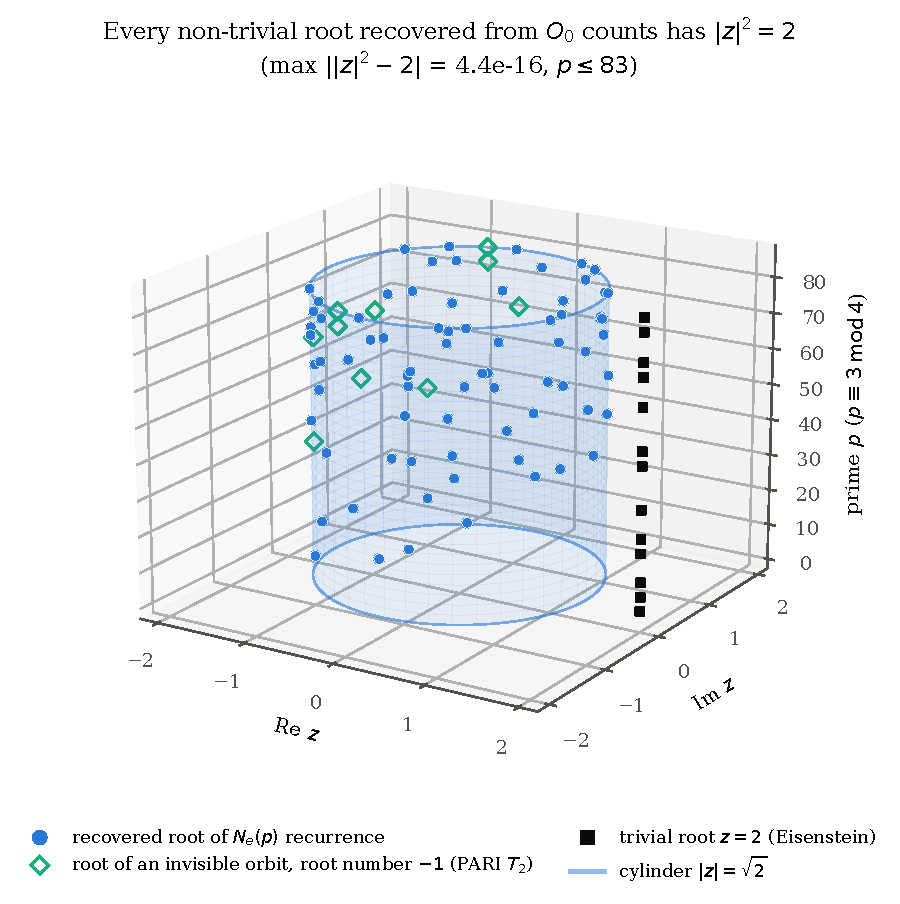
\includegraphics[width=0.78\textwidth]{fig3_ramanujan_cylinder.pdf}
\caption{Recurrence roots of $N_e(p)$, $p\le83$, recovered by Berlekamp--Massey from $\Oz$ counts (filled), drawn in the complex plane at height $p$. Hollow diamonds are the Ihara roots $z^2-a_2z+2=0$ of the orbits that $E_0$ does not see. All of these have root number $-1$ (PARI $T_2$ data); no invisible $w=+1$ orbit occurs for $p\le83$. Squares mark the trivial root $z=2$. The translucent surface is $|z|=\sqrt2$. A non-Ramanujan graph would put filled points off the cylinder.}
\label{fig:cyl}
\end{figure}

\begin{figure}[htbp]
\centering
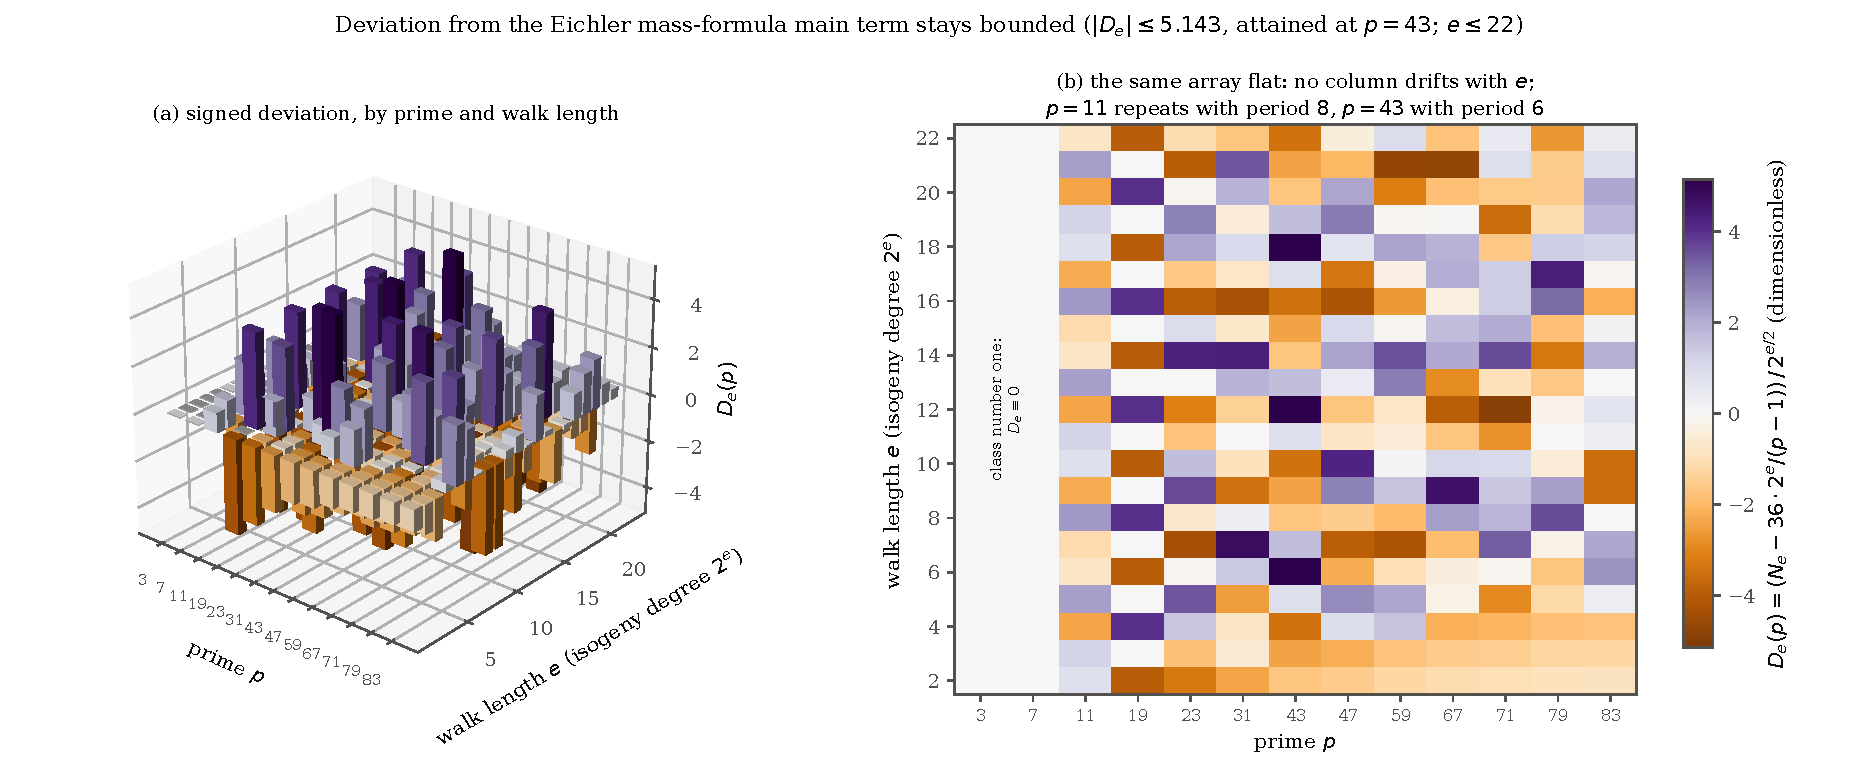
\includegraphics[width=\textwidth]{fig4_deviation_bars.pdf}
\caption{Normalised deviation $D_e(p)$ of the primitive counts from the mass-formula main term, $2\le e\le22$, in two views of the same array. (a) Signed bars in $(p,e)$. (b) The same values flat, which is the panel to read the claim off: in the 3D view front bars occlude rear ones and the identically-zero columns at class number one ($p=3,7$) are invisible as slabs. No column drifts with $e$, the extreme value is $5.143$ at $p=43$, and the exact periodicity is visible as repeating rows ($p=11$, period $8$; $p=43$, period $6$). Colour encodes the signed value on a purple--orange diverging scale with a neutral midpoint.}
\label{fig:dev}
\end{figure}

\begin{figure}[htbp]
\centering
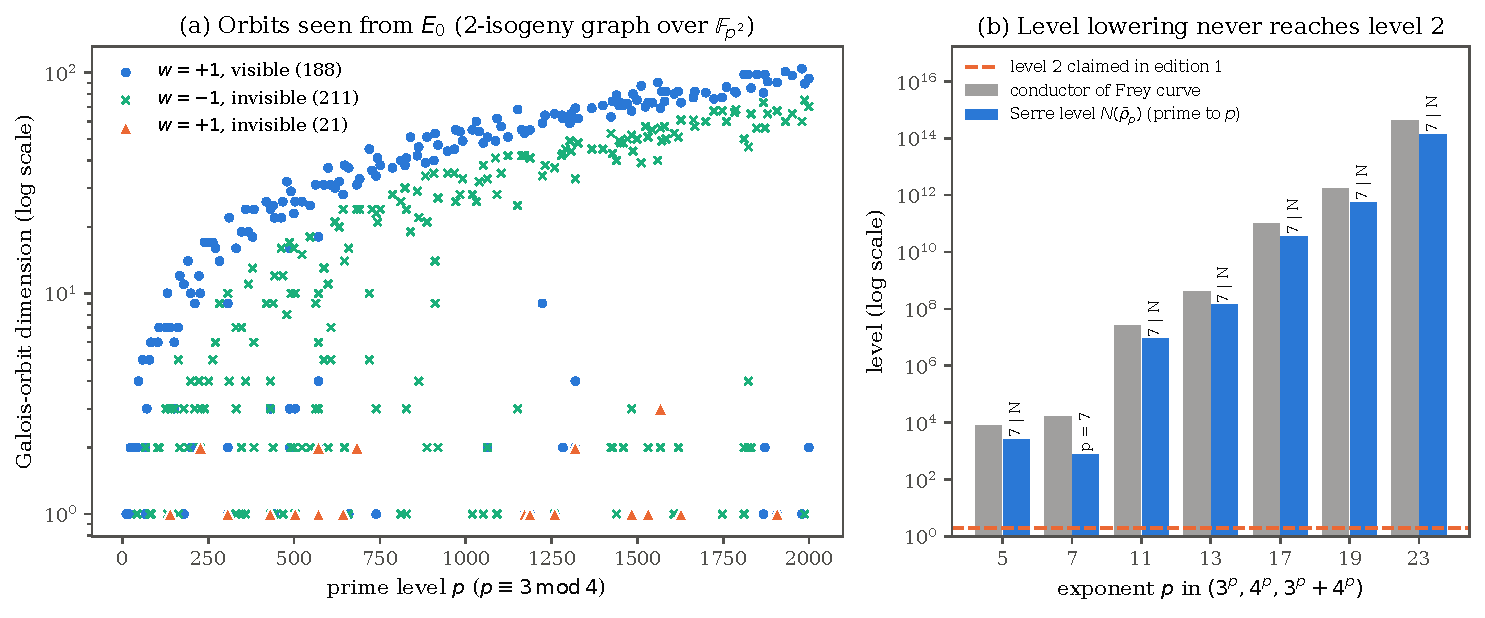
\includegraphics[width=\textwidth]{fig5_visibility_and_frey.pdf}
\caption{(a) Every cusp orbit for $p<2000$ ($p\equiv3\bmod4$), by orbit dimension. No orbit with root number $-1$ is visible from $E_0$ --- which is forced rather than observed (Section~\ref{sec:w-forced}) and is drawn here only to show the shape of the data. The 21 triangles are $w=+1$ orbits with a vanishing central value, and those are the measurement. (b) Frey curves of $(3^p,4^p,3^p+4^p)$: the conductor (grey) and the Serre level prime to $p$ (blue), on a log scale, against the level~2 claimed in edition~1 (dashed). The prime 7 divides the Serre level for every $p\neq7$.}
\label{fig:vis}
\end{figure}

\begin{figure}[htbp]
\centering
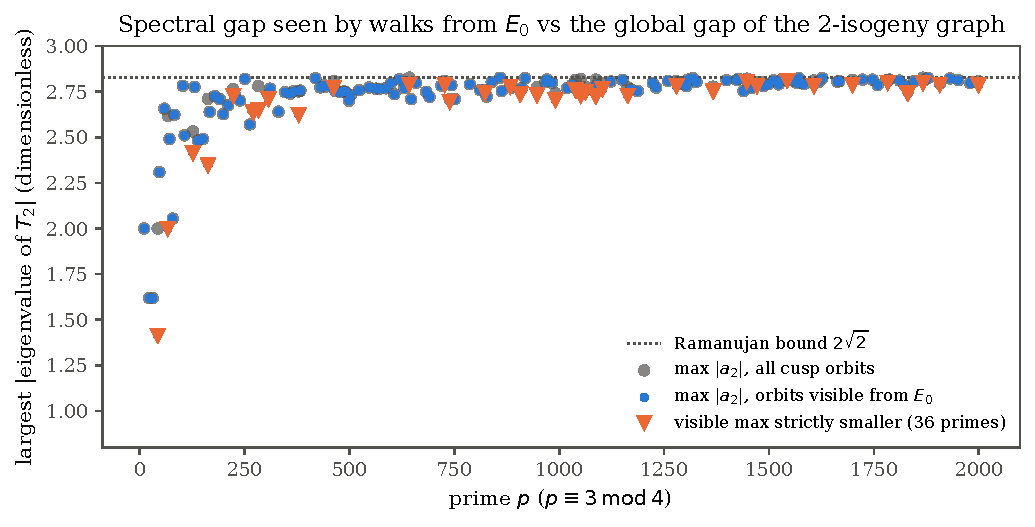
\includegraphics[width=0.85\textwidth]{fig6_spectral_gap_E0.pdf}
\caption{Largest $|a_2|$ over all cusp orbits (grey) and over the orbits visible from $E_0$ (blue), for each prime $p<2000$. Triangles mark the 36 primes where walks from $E_0$ see a strictly larger spectral gap than the global gap. All values lie below the Ramanujan bound $2\sqrt2$ (dotted).}
\label{fig:gap}
\end{figure}

\begin{figure}[htbp]
\centering
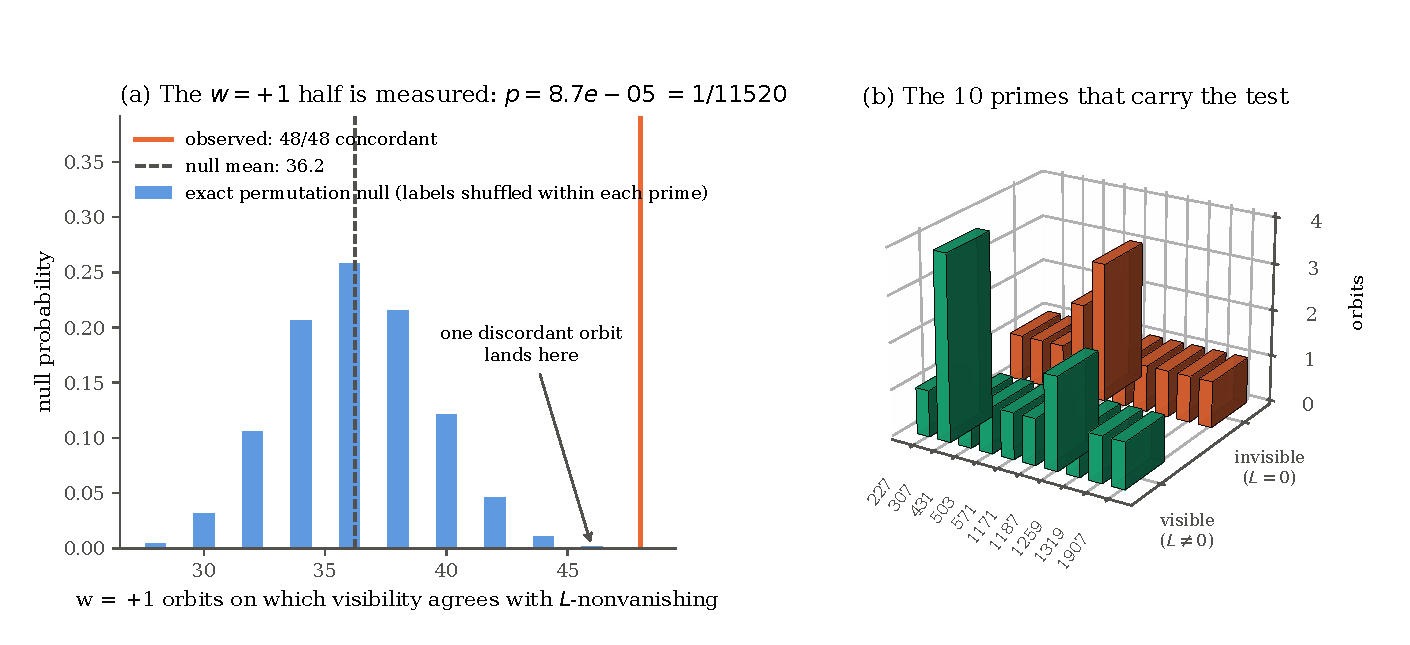
\includegraphics[width=\textwidth]{fig_forced_vs_free.pdf}
\caption{The half of P3 that carries evidence. (a) Exact permutation null of the number of $w=+1$ orbits on which graph visibility agrees with $L$-nonvanishing, with the $L$-vanishing labels reshuffled within each prime. The null is a hypergeometric convolution over the 10 primes carrying both outcomes, not a Monte Carlo sample; it centres on $36.2$ of 48. The observed value is 48, giving $p=1/11520=8.7\times10^{-5}$. The arrow marks where a single discordant orbit would fall ($p=1.6\times10^{-3}$, failing the $10^{-3}$ gate) --- the test can come out non-significant, which is what distinguishes it from the withdrawn control N(iv). (b) The ten primes that carry the test, by visibility and by whether a central value vanishes. Both outcomes occur at each of them, which is what makes the labels permutable; agreement is exact in every column. The 8 further primes whose $w=+1$ orbits are all invisible contribute no freedom and are excluded from the null.}
\label{fig:forced}
\end{figure}

\section{Serre levels of the Frey family $(3^p,4^p,3^p+4^p)$}
\label{sec:frey}
For a semistable Frey curve, a prime $l\neq p$ divides the Serre level $N(\bar\rho_p)$ iff $p\nmid v_l(\Delta_{\min})$; this is the input to Ribet's level lowering~\cite{Ribet1990}. Here $v_3(\Delta_{\min})=2p$ (stripped), $v_2(\Delta_{\min})=4p-8$ (kept), and $v_l(\Delta_{\min})=2v_l(C)$ for odd $l\mid C$. Theorem~\ref{thm:seven} keeps $7$ for every $p\ne7$. Table~\ref{tab:frey} shows the PARI data.

\begin{table}[htbp]
\centering
\caption{Frey curves of $(3^p,4^p,3^p+4^p)$ (PARI \texttt{ellglobalred}). All are semistable. The Serre level is prime to $p$. In every row the only stripped odd prime is~$3$.}
\label{tab:frey}
\footnotesize
\begin{tabular}{@{}r l l r@{}}
\toprule
$p$ & $3^p+4^p$ & conductor & Serre level (prime to $p$) \\
\midrule
5 & $7\cdot181$ & $2\cdot3\cdot7\cdot181$ & $2534=2\cdot7\cdot181$ \\
7 & $7^2\cdot379$ & $2\cdot3\cdot7\cdot379$ & $758=2\cdot379$ ($v_7(\Delta)=4$, $7\nmid4$: not finite at $7$) \\
11 & $7\cdot727\cdot859$ & $2\cdot3\cdot7\cdot727\cdot859$ & $8742902$ \\
13 & $7\cdot313\cdot31357$ & $2\cdot3\cdot7\cdot313\cdot31357$ & $137406374$ \\
17 & $7\cdot919\cdot2690659$ & $2\cdot3\cdot7\cdot919\cdot2690659$ & $34618018694$ \\
19 & $7\cdot39434309773$ & $2\cdot3\cdot7\cdot39434309773$ & $552080336822$ \\
23 & $7\cdot139\cdot72418178167$ & $2\cdot3\cdot7\cdot139\cdot72418178167$ & $140925774712982$ \\
\bottomrule
\end{tabular}
\end{table}

\section{Scope and limitations}
\label{sec:scope}
\begin{itemize}
  \item Nothing in this paper verifies SQIsign, any signature scheme, or any security property. The Rust crate checks a norm (Table~\ref{tab:probe}), and no timing was measured.
  \item P1--P3 are known theorems. The contribution is a reproducible computational test of them for $\Oz$, and the observation about the gap seen from $E_0$. It is not a proof. The Lean files prove elementary algebra: the Ihara lemma, the norm forms, the halving lemma, the corrections, the Serre-level valuation, and --- new in this edition --- the two forcing arguments that establish which half of P3 carries evidence (Section~\ref{sec:lean-forced}). The Deuring correspondence, Gross's formula, Eichler--Shimura and Deligne are not formalised. They enter only through the computation, and the forcing theorems are explicitly conditional on them.
  \item ``Vanishing'' of an $L$-value means $|L|<10^{-20}$ at 38 digits, with every functional-equation check below $-30$ bits. The observed zeros are below $2\times10^{-38}$. This is numerical evidence, not a proof that the value is zero. The statements about $L(f,1)=0$ concern analytic rank only.
  \item The tested ranges are $p\le83$ and $e\le22$ (lattice), $e\le48$ (graph), $p<2000$ (visibility), $p<700$ (the independent modular-symbol check), and orbits of dimension $\le3$ (the $L$-values). The $L$-value test covers 48 orbits with $w=+1$, not all 209.
  \item The class-number-one laws are kernel-checked for $e=1,2$ only. The statement $N_e=r(2^e)-r(2^{e-2})$ is proved as a halving lemma, not as a \texttt{Finset} bijection.
  \item The Frey-curve semistability theorem (Theorem~\ref{thm:frey}) is the coprimality statement. Minimality and the reduction types come from PARI and are not formalised.
  \item The PARI computations ran in an isolated Python environment with \texttt{cypari2}, because neither \texttt{gp} nor Sage is installed system-wide on the build host. The script takes that interpreter from \texttt{PAPER\_C\_PARI\_PYTHON}.
\end{itemize}

\section{Research directions}
\label{sec:directions}
\textbf{Statistics of exceptional invisibility.} Extend the visibility test to $p<10^4$. Compare the rate of $w=+1$ orbits invisible from $E_0$ (21 of 209 below $2000$, split between $L(f,1)=0$ and $L(f\otimes\chi_{-4},1)=0$) with random-matrix predictions for the vanishing of quadratic-twist central values.
\textbf{A base point that can falsify the $w=-1$ half of Gross's formula.} Every claim about root-number-$-1$ invisibility made from $E_0$ is forced by $j(E_0)\in\mathbb F_p$ (Section~\ref{sec:w-forced}). To turn it back into a measurement, repeat the visibility test from a supersingular $j\in\mathbb F_{p^2}\setminus\mathbb F_p$, where $Fe_j\ne e_j$ and the projection onto a $w=-1$ orbit is no longer forced to vanish by symmetry. Gross's formula still predicts invisibility there, through $L(f,1)=0$, so what the experiment buys is a prediction that could come out false rather than one closed off by two independent arguments: a visible $w=-1$ orbit would refute the dictionary. The same test distinguishes properties of SQIsign's chosen base point from properties of the graph.
\textbf{Starting-curve-specific mixing.} Quantify how much faster random $2^e$-walks from $E_0$ equidistribute than the global gap predicts, at the 36 primes where the visible gap is larger. Do the same for $j=0$ with $p\equiv2\bmod3$ and $\chi_{-3}$.
\textbf{An honest toy verifier.} Replace the norm check with a real isogeny-walk verifier over $\mathbb F_{p^2}$ for small $p$ (V\'elu formulas, explicit kernels). Ship negative tests that reject $[2^k]$, backtracking responses and wrong codomains, and measure timing with dudect-style tests instead of asserting it.
\textbf{Lean.} Prove the \texttt{Finset} bijection $N_e=r(2^e)-r(2^{e-2})$, the class-number-one laws for all $e$, and a statement that links recurrence roots to \lean{ihara_circle}. The Deuring correspondence would enter as a hypothesis. A sharper target is suggested by Section~\ref{sec:lean-forced}: discharge the hypotheses of \lean{frobenius_forces_vanishing} for the actual Brandt module --- that $F$ permutes the supersingular basis, commutes with every $B(\ell)$, and acts by $a_f(p)$ on the $f$-component --- which would turn the forcing from a conditional statement into a theorem about the graph. That is a formalisation of a known piece of Eichler theory, not of Gross's formula, so it is within reach in a way the rest of the dictionary is not.
\textbf{Serre levels of Hellegouarch families.} Characterise, via lifting the exponent, which odd primes always survive for $(x^p,y^p,x^p+y^p)$; for example, primes dividing $x+y$ with $p\nmid2(v(x+y)+v(p))$. Do this without claiming anything of Fermat strength.

\section*{Data and code availability}
The following files are in this repository; the Zenodo bundle lists them.
\begin{itemize}
  \item Manuscript: \path{papers/three_breakthroughs/paper_c/PaperC_FLT_Modular_PQC_SQIsign_Quantum_Rust_Lean4.tex}.
  \item Results: \path{paper_c_v2_results.json}; Lean gate record: \path{paper_c_v2_lean_gate.json}.
  \item Figures: \path{fig3_ramanujan_cylinder.pdf}, \path{fig4_deviation_bars.pdf}, \path{fig5_visibility_and_frey.pdf}, \path{fig6_spectral_gap_E0.pdf}.
  \item Scripts: \path{scripts/three_breakthroughs/paper_c_v2_experiment.py}, \path{paper_c_v2_pari_worker.py}, \path{paper_c_v2_figures.py}, and the probe crate \path{paper_c_v2_rust_probe}.
  \item Lean: \path{formal/ANSE/PaperC_DeuringSpectrum.lean}, \path{formal/ANSE/PaperC_ForcedVisibility.lean}, \path{formal/ANSE/Breakthroughs3Domains.lean}, \path{formal/ANSE/Breakthroughs3DomainsSpec.lean} and \path{formal/ANSE/ElenchusTrilogySpec.lean}.
\end{itemize}

\begin{thebibliography}{99}
\bibitem{BuzzardTaylor} K.~Buzzard and R.~Taylor, ``Towards a Lean proof of Fermat's Last Theorem'' (blueprint), Imperial College London; repository \url{https://github.com/ImperialCollegeLondon/FLT}.
\bibitem{DeFeo2020} L.~De~Feo, D.~Kohel, A.~Leroux, C.~Petit, and B.~Wesolowski, ``SQIsign: Compact post-quantum signatures from quaternions and isogenies,'' in \emph{Advances in Cryptology --- ASIACRYPT 2020}, Springer, pp.~64--93, 2020.
\bibitem{SQIsignSpec} The SQIsign team, SQIsign specification and reference implementation, \url{https://sqisign.org}.
\bibitem{Deuring1941} M.~Deuring, ``Die Typen der Multiplikatorenringe elliptischer Funktionenk\"orper,'' \emph{Abh.\ Math.\ Sem.\ Univ.\ Hamburg}, vol.~14, pp.~197--272, 1941.
\bibitem{Kohel1996} D.~Kohel, \emph{Endomorphism Rings of Elliptic Curves over Finite Fields}, Ph.D.\ thesis, University of California, Berkeley, 1996.
\bibitem{Gross1987} B.~H.~Gross, ``Heights and the special values of $L$-series,'' in \emph{Number Theory (Montreal, 1985)}, CMS Conf.\ Proc., vol.~7, Amer.\ Math.\ Soc., pp.~115--187, 1987.
\bibitem{Voight} J.~Voight, \emph{Quaternion Algebras}, Graduate Texts in Mathematics 288, Springer, 2021; \url{https://jvoight.github.io/quat.html}.
\bibitem{Pizer1990} A.~K.~Pizer, ``Ramanujan graphs and Hecke operators,'' \emph{Bull.\ Amer.\ Math.\ Soc.}, vol.~23, no.~1, pp.~127--137, 1990.
\bibitem{Ribet1990} K.~A.~Ribet, ``On modular representations of $\operatorname{Gal}(\overline{\mathbb{Q}}/\mathbb{Q})$ arising from modular forms,'' \emph{Invent.\ Math.}, vol.~100, pp.~431--476, 1990.
\bibitem{LMFDB} The LMFDB Collaboration, \emph{The L-functions and Modular Forms Database}, newform 11.2.a.a, \url{https://www.lmfdb.org/ModularForm/GL2/Q/holomorphic/11/2/a/a/}.
\bibitem{PARI} The PARI~Group, \emph{PARI/GP version 2.17.2}, Univ.\ Bordeaux, \url{https://pari.math.u-bordeaux.fr/}.
\bibitem{Mathlib} The mathlib Community, ``The Lean mathematical library,'' in \emph{Proc.\ 9th ACM SIGPLAN Int.\ Conf.\ on Certified Programs and Proofs (CPP 2020)}, pp.~367--381, 2020.
\end{thebibliography}

\end{document}
